\section*{Results}

Here I discuss only the directly relevant parameters and metrics. The graphs of \verb|dev-accuracy| during training and \verb|train-loss| that are satandard and do not proide much of an insight for the given parameters, are saved in the \verb|./plots/| directory.

\subsection*{Feed Forward Neural Network}

I trained and evaluated multiple models on the \verb|en-atis| dataset. The results for the top 5 models are shown below, with metrics over the 5 metrics, Accuracy, Precision, F1-Macro, F1-micro, Recall Score 

% Model Name                                         | Accuracy   | Precisio   | F1-macro   |  F1-micro   | Recall    
% EvaluationFFNN-p=2_s=1_n=1_p=2_s=1_n=1_128         | 98.7234   % | 98.7492% | 97.1516% | 98.7234% | 98.7234%
% EvaluationFFNN-p=2_s=1_n=2_p=2_s=1_n=2_128_64      | 98.7234   % | 98.7398% | 97.103 % | 98.7234% | 98.7234%
% EvaluationFFNN-p=2_s=1_n=1_p=2_s=1_n=1_32          | 98.6474   % | 98.6779% | 96.9825% | 98.6474% | 98.6474%
% EvaluationFFNN-p=3_s=1_n=2_p=3_s=1_n=2_128_64      | 98.6322   % | 98.6417% | 96.7312% | 98.6322% | 98.6322%
% EvaluationFFNN-p=3_s=1_n=1_p=3_s=1_n=1_64          | 98.617    % | 98.6312% | 96.8527% | 98.617 % | 98.617 %

% Create a table to display the above metrics :

\begin{table}[h]
    \centering
\begin{tabular}{|c|c|c|c|c|c|}
\hline
Model Name & Accuracy & Precision & F1-macro & F1-micro & Recall \\
\hline 
p=2 s=1 n=1 : [128] & \textbf{98.7234\%} & \textbf{98.7492\%} & \textbf{97.1516\%} & \textbf{98.7234\%} & \textbf{98.7234\%}\\
\hline
p=2 s=1 n=2 : [128,64] & 98.7234\% & 98.7398\% & 97.103\% & 98.7234\% & 98.7234\% \\
\hline 
p=2 s=1 n=1 : [32] & 98.6474\% & 98.6779\% & 96.9825\% & 98.6474\% & 98.6474\% \\
\hline 
p=3 s=1 n=2 : [128,64] & 98.6322\% & 98.6417\% & 96.7312\% & 98.6322\% & 98.6322\% \\ 
\hline 
p=3 s=1 n=1 : [64] & 98.617\% & 98.6312\% & 96.8527\% & 98.617\% & 98.617\% \\
\hline
\end{tabular}
\end{table}

The best performing model is therefore obtained for the \verb|p=2 s=1 n=1:[128]|, which is shown in the table above. It also achieves the best scores in all the other metrics the models are evaluated on.

The confucsion metric for the model is given below:

\begin{figure}[h]
    \centering
    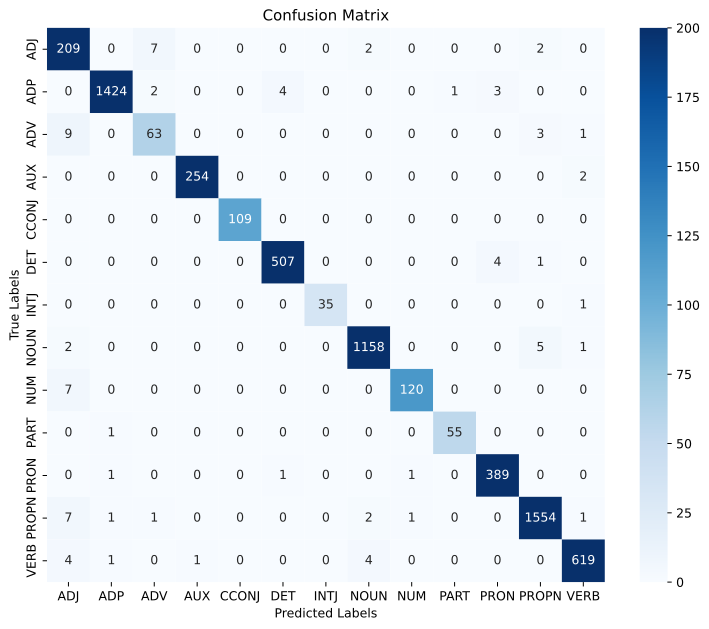
\includegraphics[width=0.8\textwidth]{../pictures/ConfusionMatrixBestFFNN.png}
    \caption{Confusion Matrix}
\end{figure}

\subsubsection{Remarks}
The models simplicity in the number of layers and context window seemed to have struck a nice balance with the large size of the hidden layer to optimize its performance for the given task.

Also, the top 3 models are the same, if measured across any of these metrics, and the common hyperparameter among all these is \verb|p=2, s=1|. Hinting that a simplistic, and \textit{past-biased} model tends to perform better on \verb|POS tagging|.


\subsection*{Recurrent Neural Networks}

I trained and evaluated approximately 150 models for hypereparameter tuning. The results for the top 5 models are as follows :

% Model Name                                         | Accuracy | Precision | F1-macro | F1-micro | Recall    
% EvaluationRNN-s=3_h=1_b=True_l=64_n=3_h=64_bidirec | 98.7994% | 98.836%   | 90.0127% | 98.7994% | 98.7994%
% EvaluationRNN-s=2_h=2_b=True_l=64_n=2_h=64_bidirec | 98.7538% | 98.7542%  | 97.0912% | 98.7538% | 98.7538%
% EvaluationRNN-s=2_h=2_b=True_l=128_n=2_h=128_bidir | 98.7234% | 98.7434%  | 96.6337% | 98.7234% | 98.7234%
% EvaluationRNN-s=3_h=2_b=True_l=64_n=3_h=64_bidirec | 98.7082% | 98.7156%  | 97.344 % | 98.7082% | 98.7082%
% EvaluationRNN-s=2_h=2_b=True_l=64_n=2_h=64_bidirec | 98.693%  | 98.7206%  | 89.6664% | 98.693 % | 98.693 %

\begin{table}[h]
\centering
\begin{tabular}{|l|l|l|l|l|l|}
\hline
Model Name & Accuracy   & Precision   & F1-macro   &  F1-micro   & Recall    \\ \hline
$s=3, b=True, h=64, l = 1 : [64]$  & \textbf{98.7994\%} & \textbf{98.836\%} & 90.0127\% & \textbf{98.7994\%} & \textbf{98.7994\%} \\ \hline
$s=2, b=True, h=64, l = 2 : [128, 64] $ & 98.7538   \% & 98.7542\% & 97.0912\% & 98.7538\% & 98.7538\% \\ \hline
$s=2, b=True, h=128, l = 2 : [128, 64] $ & 98.7234   \% & 98.7434\% & 96.6337\% & 98.7234\% & 98.7234\% \\ \hline
$s=3, b=True, h=64, l = 2 : [64, 64]$ & 98.7082   \% & 98.7156\% & \textbf{97.344\%} & 98.7082\% & 98.7082\% \\ \hline
$s=2, b=True, h=64, l = 2 : [64, 64]$ & 98.693    \% & 98.7206\% & 89.6664\% & 98.693 \% & 98.693 \% \\ \hline
\end{tabular}
\end{table}

Here $s$ denotes the stack size of the RNN, $b$ denotes if the RNN is bidirectional, $h$ denotes the hidden state size, and $l$ denotes the number of layers in the classifier, followed by the layer sizes themselves.

\subsubsection{Remarks}
Similar to the FFNN models, the RNN models underwent extensive hyperparameter tuning to achieve optimal performance. Notably, the model with parameters \verb|s=3, b=True, h=64, l=1 : [64]| outperformed others in terms of accuracy and precision, albeit with a slightly lower F1-macro score compared to some other models. This is due to the class \verb|SYM| that has just a single point, predicting that incorrectly costs the model heavily.

Confusion Matrix of the best performing model : 

\begin{figure}[h]
\centering
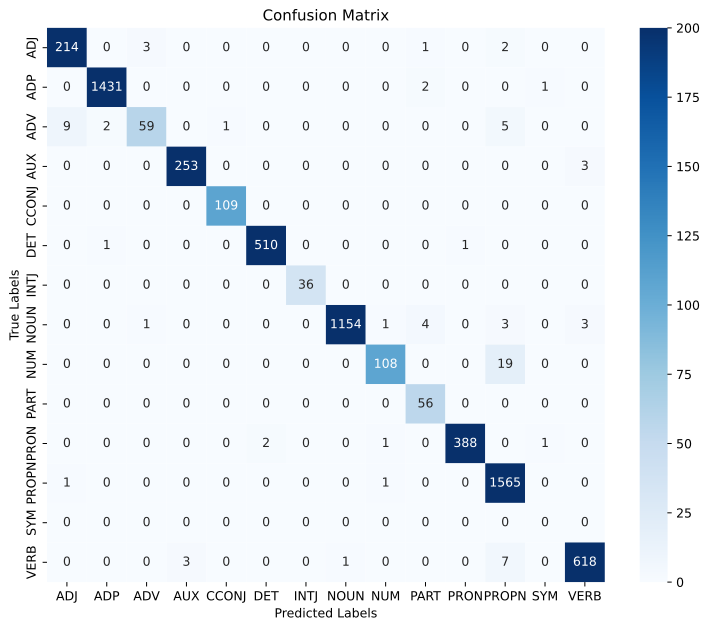
\includegraphics[width=0.8\textwidth]{../pictures/ConfusionMatrixBestRNN.png}
\caption{Confusion Matrix of the best performing model}
\end{figure}

The bidirectional nature of certain models ($b=True$) seems to contribute positively to their performance, especially when combined with larger hidden state sizes. However, it's crucial to note that in some cases, increasing the complexity of the model (such as adding more layers or increasing hidden state sizes) did not necessarily lead to improved performance across all metrics.

Additionally, as seen in the top-performing models, a shallower architecture with fewer layers but appropriately sized hidden states ($l=1$) can sometimes yield competitive results, emphasizing the importance of balancing model complexity with dataset characteristics.
